\documentclass[11pt]{beamer}
% \usepackage[T1]{fontenc}
% \usepackage[utf8]{inputenc}

% \usepackage{pgf,pgfpages}

% \usepackage{tikz}
% \usetikzlibrary{arrows,shapes,backgrounds,calc}

% \usepackage{graphicx}
% \usepackage{colortbl}
% \usepackage{units}

% % \usepackage{calrsfs}
% % \DeclareMathAlphabet{\pazocal}{OMS}{zplm}{m}{n}
% % \usepackage{calligra}
% \usepackage[cal=boondox]{mathalfa}
% % \usepackage{bickham}
% % \usepackage{boondox-cal}
% % \usepackage{boondox-calo}
% % \usepackage{dutchcal}

% %% Beamer style >>>>>>>>>>>>>>>>>>>>>>>>>
% \mode<presentation>
% {
%   \usetheme{PHD}
%   \setbeamercovered{transparent}
%   \setbeamertemplate{items}[square]
% }

% %\usefonttheme[onlymath]{serif}

% \beamertemplatenavigationsymbolsempty

% \defbeamertemplate{enumerate item}{mycircle}
% {
%   %\usebeamerfont*{item projected}%
%   \usebeamercolor[bg]{item projected}%
%   \begin{pgfpicture}{0ex}{0ex}{1.5ex}{0ex}
%     \pgfcircle[fill]{\pgfpoint{-0.1pt}{.65ex}}{1.1ex}
%     \pgfbox[center,base]{\color{PHDyellow}{\insertenumlabel}}
%   \end{pgfpicture}%
% }
% [action]
% {\setbeamerfont{item projected}{size=\scriptsize}}
% \setbeamertemplate{enumerate item}[mycircle]

% %<<<<<<<<<<<<< beamer style

% \title[DG Approximations to Anisotropic Stokes]{Discontinuous Galerkin
%   Approximation of Anisotropic Viscous Flows}
% \author[J.R. Rodr\'{\i}guez Galv\'an]{\em J. Rafael Rodr\'{\i}guez
%   Galv\'an\vspace{-0.9em}} \date{\footnotesize\structure{\em
%     Doc-Course: ``Partial Differential Equations: Analysis, Numerics
%     and Control''} \\[1ex] Granada. April 25, 2018}

% % XeLaTeX font choosing
% % \usepackage{fontspec}%{xltxtra} %fontspec}
% % \setsansfont{Fontin Sans}
% % \setsansfont{Lato}

% % PDFLaTeX font choosing
% %\usepackage[default, scale=1.0]{lato}

% \setbeameroption{hide notes} % Only slides
% % \setbeameroption{show only notes} % Only notes
% % \setbeameroption{show notes on second screen=right} % Both

% % Different math fonts, see http://tug.org/pracjourn/2006-1/hartke/hartke.pdf
% %\usepackage{eulervm}
% %\usepackage{ccfonts, eulervm}
% %\usepackage[math]{kurier}
% %\usepackage[math]{anttor}
% %\usepackage{pxfonts}
% %\usepackage{mathpazo}
% %\usepackage{mathpple}
% %\usepackage[varg]{txfonts}
% %\usepackage{arev}
% %\usepackage{fourier}

% \usepackage{tabularx}
% \usepackage{array, multirow, booktabs, rotating} % booktabs: toprule, midrule...

% \newcommand{\heatProblem}{(Heat-Problem)\xspace}
% \newcommand{\poissonProblem}{(Poisson-Problem)\xspace}

% \usepackage{presenta-granada-2018}

% \newtheorem{remark}{Remark}
% \newtheorem{proposition}{Proposition}
% %\newtheorem{theorem}{Theorem}

% % Presentation goodies >>>>>>>>>>>>>>>>>>>>>>>>>>>>
% \newcommand<>{\myframed}[1]{\alt#2{\tikz[phd] \node[box] {#1};}{{#1}}}
% \newcommand<>{\myframedAlert}[1]{\alt#2{\tikz[phdB] \node[boxB] {\color{black}#1};}{{#1}}}
% \newcommand<>{\framedmath}[1]{%
% \alt#2{\tikz[phd] \node[box] {\ensuremath{#1}};}{\ensuremath{#1}}}
% \newcommand{\framedB}[1]{\tikz[phd] \node[boxB] {#1};}
% \newcommand{\framedmathB}[1]{\framedB{\ensuremath{\displaystyle{#1}}}}
% \newcommand{\ver}[1]{\footnote{See #1}}
% \newcommand{\cita}[1]{{\color{PHDgray}\cite{#1}}}
% \newcommand\cellalert[2]{\only<#1>{\cellcolor{PHDyellow}}\alt<#1>{\textbf{#2}}{#2}}
% \newcommand{\soften}[1]{{\color{PHDgray}#1}}
% \newcommand{\rowalert}[7]{%
%     \cellalert{#1}{#2} & \cellalert{#1}{#3} &
%     \cellalert{#1}{#4} & \cellalert{#1}{#5} &
%     \cellalert{#1}{#6} & \cellalert{#1}{#7}}

% \newcommand{\kk}{\Delta t}
% % \usepackage{wasysym}
% % \newcommand{\good}{{\color{PHDgreen}$\CIRCLE$}} %\blacksmiley
% % \newcommand{\bad}{{\color{PHDred}$\CIRCLE$}}
% \usepackage{pifont}
% \newcommand{\good}{{\color{PHDgreen}\ding{52}}}
% \newcommand{\bad}{{\color{PHDred}\ding{56}}}
% \newcommand{\exclamation}{{\large\color{PHDred}{\textbf{\itshape !}}}}
% \newcommand{\question}{{\large\color{PHDred}{\textbf{\itshape ?}}}}
% \newcommand\colorUnderLine[2][PHDyellow]{\color{#1}\underline{{\color{black}#2}}\color{black}\xspace}
% \newcommand\gris{\color{PHDgray}}
% \newcommand\amarillo{\color{PHDyellow}}
% \newcommand\tiragris[1]{{\par\hfill\small\gris{#1}}}
% %<<<<<<<<<<<<<<<

% \setcounter{tocdepth}{1}


% %
% % Bibliography
% %
% %\usepackage{natbib}

% % To list each bibliographic entry in a line
% \setbeamertemplate{bibliography entry title}{}
% \setbeamertemplate{bibliography entry location}{}
% \setbeamertemplate{bibliography entry note}{}

% % ... end of preamble.

% \AtBeginSection{\frame{\sectionpage}}

% \renewcommand{\vv}{v}
% \renewcommand{\VV}{V}

%======================================================================
\begin{document}
%======================================================================

% % Tikz style and beamer template ------->>>
% \tikzstyle{every picture}+=[remember picture]
% \tikzstyle{na} = [baseline=-.5ex]
% \tikzstyle{phd} = [baseline=-.6ex,
%   box/.style={rectangle, draw=PHDblueC, thick, fill=PHDblueA,
%     align=center, rounded corners, minimum height=1.6em},
%   boxB/.style={rectangle, draw=PHDredA, thick, fill=PHDblueA,
%     align=center, rounded corners, minimum height=1.6em}]
% \tikzstyle{phdB} = [baseline=-.7ex,
%   box/.style={rectangle, draw=PHDblueC, thick, fill=PHDblueA,
%     align=center, rounded corners, minimum height=1.6em},
%   boxB/.style={rectangle, draw=PHDredA, thick, fill=PHDblueA,
%     align=center, rounded corners, minimum height=1.6em}]
% \tikzstyle{myarrow} = [->,>=latex, PHDredA, shorten >=4pt,
%   opacity=.6, line width=0.6mm]
% \tikzstyle{myarrow2} = [->,>=latex, PHDblueC, shorten >=4pt, opacity=.2, line width=0.4mm]
% \tikzstyle{myarrow3} = [
%      opacity=.7,
% %    >=triangle 60,              % Nice arrows; your taste may be different
%     node distance=6mm and 60mm, % Global setup of box spacing
%     every join/.style={norm},   % Default linetype for connecting
%                                 % boxes
%     line width=0.6mm,
%     PHDredA,
%     ->
%     ]
% \setbeamertemplate{background}
%  {
\includegraphics[width=\paperwidth,height=\paperheight]{frontpage_bg}}
% \setbeamertemplate{footline}[default]
% % <<<-------


% % Write custom titlepage ------->>>
% \begin{frame}
%   \titlepage
%   \vspace{5cm}
% \end{frame}

% % Set the background for the rest of the slides.
% \setbeamertemplate{background}
%  {
\includegraphics[width=\paperwidth,height=\paperheight]{slide_bg}}


% % Write all of the slides..........

% \begin{frame}{Outline}
%   \tableofcontents
% \end{frame}

% % Start inserting infoline at the end
% \setbeamertemplate{footline}[PHDtheme]
% % <<<-------

% \newcommand{\imgdir}{Undefined, use renewcommand!}

% %============================================================================
% \section{Preliminary Concepts and Notation}
% %============================================================================



% \begin{frame}{Sobolev Spaces}
%   \small
%   \medskip
%   $W^{s,p}(\Omega)=\big\{u\in D'(\Omega):\ \partial^\alpha u \in L^p(\Omega),\ |\alpha|\le s\big\}$
%   \bigskip
% \begin{itemize}\itemsep1em
% \item Particular case \alert{$p=2$}:
%   $$
%   \alert{H^s(\Omega)}:=W^{s,\alert{2}}(\Omega)=\big\{u\in D'(\Omega):\
%   \partial^\alpha u \in L^{\alert{2}}(\Omega),\ |\alpha|\le s\big\}
%   $$
%   \vspace{-1em}
%   \begin{itemize}
%   \item Hilbert space with scalar product and norm:
%     $$
%     (u, v)_s = \sum_{|\alpha|\le s}\int_\Omega \partial^\alpha u \partial^\alpha v,
%     \qquad
%     \norm[s]{u} = +\sqrt{ (u,u)_s }
%   ~\vspace{-1em}~
%     $$
%   \end{itemize}
% \item For instance,
%   \begin{align*}
%     \alert{H^0(\Omega)}&=L^2(\Omega), \quad (u,v)_0=(u,v)_{L^2(\Omega)}, \quad \norm[0]{u}=\norm[L^2(\Omega)]{u}
%     \\[0.5em]
%   \alert{H^1(\Omega)}&=\big\{u\in L^2(\Omega):\
%   \partial_i u \in L^{{2}}(\Omega),\ 1\le i \le d\big\}
%     \\
%     &(u, v)_1 %= \int_\Omega u\,v + \sum_{i=1}^d \int_\Omega \partial_i u \partial_i v
%     = \int_\Omega u\,v +  \int_\Omega \grad u \grad v
%     \\
%     &\norm[1]{u} = \left(\int_\Omega \norm[0]{u}^2 + \int_\Omega \norm[0]{\grad u}^2\right)^{1/2}
%   \end{align*}

% \end{itemize}
% \end{frame}


% \begin{frame}{Sobolev Embedding}
%   \begin{theorem}
%     For $\Omega\subset\Rset^d$, we have:
%     $$
%     H^s(\Omega)\subset C^r(\Omega) \quad \text{if}\quad \frac12 < \frac{s-r}d
%     $$
%   \end{theorem}
%   In particular,
%   $$
%   H^s \subset C^0(\Omega) \quad \text{if}\quad
%   \left\{
%     \begin{aligned}
%     s>\frac12 \quad \text{for}\quad d=1
%     \\
%     s> 1 \quad \text{for}\quad d=2
%     \\
%     s>\frac32 \quad \text{for}\quad d=3
%   \end{aligned}
%     \right.
%   $$
% % \begin{itemize}\itemsep1em
% % \end{itemize}
%   \small
%   \color{gray}
%   \textbf{Remark}:  Sobolev spaces with \textbf{fractional indices} $H^{s+1/2}(\Omega)$
%   can be defined by interpolating between $H^s(\Omega)$ and $H^{s+1}(\Omega)$,
%   so that they verify
%   $$
%   H^s(\Omega) \subset H^{s+1/2}(\Omega) \subset H^{s+1}(\Omega).
%   $$
% \end{frame}


% \begin{frame}{Trace Theorems}
%   % We define $H^1_0(\Omega)=\overline{D(\Omega)}^{H^1(\Omega)}$
% % Using distributional derivatives, we can formulate partial differential equations in the dis-
% % tributional sense. The notion of traces [81] is used to define the restriction of a Sobolev
% % function along the boundary of the domain. This is important for properly defining boundary
% % conditions.
%   \begin{itemize}
%   \item Let $\gamma_0:C^0(\overline\Omega)\to C^0(\partial\Omega)$, be
%     the \alert{\bf trace} operator, \alert{$\gamma_0(v)=v|_{\partial\Omega}$}
%   \item $\gamma_0$ can be continuously extended to $H^1(\Omega)$:
%   \end{itemize}
%   \begin{theorem}
%     Let $\Omega$ be a Lipschitz open bounded set
%     \begin{enumerate}
%     \item The extended trace operator,
%       $\gamma_0:H^1(\Omega)\to H^{1/2}(\partial\Omega)$ is
%       surjective
%     \item Moreover, the kernel of $\gamma_0$ is the set $H^1_0(\Omega)=\overline{D(\Omega)}^{H^1(\Omega)}$
%     \end{enumerate}
%   \end{theorem}
%   \textbf{Remark}
%   \begin{itemize}
%   \item Statement (2) means that $H^1_0(\Omega)=\{ v \in H^1(\Omega):\ v=0\ \text{on}\ \partial\Omega\}$.
%   \item Important trace inequalities that are frequently used in the analysis of
% the DG methods: (...)
%   \end{itemize}
% \end{frame}


% \begin{frame}{Meshes}
%   Notation: \medskip
%   \begin{itemize}\itemsep1em
%   \item \structure{$\Th$}: \alert{mesh} of $\Omega$,
%     $\Th = \{K_i\}_{i=1}^{N_t} \subset\Rset^d$ (``elements'' or
%     ``triangles'')
%     \medskip
%     \begin{itemize}\itemsep0.4em
%     \item $h_K:=\text{diam}(K)$, $h:=\max_{K\in\Th}(h_K)$
%     \item Form simplicity, we consider \structure{conforming} meshes
%       \structure{(not neccessary!)}
%       \note[item]{\textbf{Conforming meshes}: For simplicity,
%         we assume that the intersection of two elements is either empty, a
%         vertex, an edge, or a face}
%     \item Assume $\Th$ is \structure{regular}, ie:\vspace{-0.5em}
%       $$\exists\rho:\quad \frac{h_K}{\rho_K} \le \rho
%       \qquad  (\rho_K=\text{radius of ball in K} )
%       $$
%     \end{itemize}

%   \item \structure{$\Eh$}: set of \alert{edges} ($d=2$) or faces ($d=3$)
%     \llaveizq{\structure{$\Ehi$}: interior faces,\\[0.3em] \structure{$\Ehb$}: boundary faces}
%     \begin{itemize}\itemsep0.5em

%     \item We associate a unit normal vector $\nn_e$ to each edge $e$
%     \item $h_e:=\text{diam}(e)$
%     \item Relation: $\forall e\subset \partial K$, \quad
%       \alert{$h_e \le C\; h_K^{d-1}$}
%       \begin{flushright}\footnotesize
%         \color{gray}due to regularity of $\Th$ and to the fact
%           {$|e| \le h_K^{d-1}$},
%           \\ $|e|:=$ length/area of edge/face $e$
%       \end{flushright}
%     \end{itemize}
%   \end{itemize}
% \end{frame}


% \begin{frame}{Broken Sobolev Spaces}
% \note[item]{Broken Sobolev spaces are natural spaces to work with the DG methods. These spaces
%   depend strongly on the partition of the domain}
% \begin{itemize}\itemsep0.7em
% \item \textit{Broken} Sobolev space:
%     \begin{equation*}
%       \alert{H^m(\Th)} := \big\{ u\in L^2(\Omega) \ |\ u\in H^m(K),\ \forall K\in\Th \big\},
%     \end{equation*}

%     {\small Scalar product and norm:}\medskip
%     \begin{itemize}\itemsep0.3em
%     \item $\prodBroken[H^s(\Th)]{u,v }= \sum_{K\in\Th}\prodEsc[H^s(K)]{u,v}$
%     \item $\normBroken[H^s(\Th)]{u}=\left(\sum_{K\in\Th}\norm[H^s(\Omega)]{u}^2 \right)^{1/2}$
%     \end{itemize}

%   \item Clearly, $H^m(\Omega)\subset H^m(\Th)$

%   \item Particular  case: broken or \structure{\textbf{discontinuous polynomials}} finite-dimensional spaces
%     $$
%     \Vh=\alert{\Pd{k}(\Th)}=\left\{ v\in L^2(\Omega):\ v|_K\in \P{k}(K),\ \forall K\in\Th \right\}
%     $$
%   % \item Discontinous finite-dimensional subspace of $H^m(\Th)$:
%   %   $$
%   %   \structure{\Pd k(\Th)}:=
%   %   \left\{
%   %     u\in L^2(\Omega) \ | \ u\in \P{k}(K), \ \forall K\in\Th \right \}.
%   %   $$
%     % \begin{flushright}
%     %   \footnotesize
%     %   \color{gray} Polinomials of degree at most $k$
%     % \end{flushright}
%     \begin{itemize}
%     \item Discontinuity along the \textbf{edges} (or faces)
%     \end{itemize}
%   \end{itemize}
% \end{frame}

% \begin{frame}{Jumps and averages}
%   Let $\alert{v}\in H^m(\Th)$  \quad (\ $\Rightarrow$\ \alert{trace} of $v$ in any $K\in\Th$ is well defined\ )
%   \bigskip
%   \begin{itemize}\itemsep1em
%   \item If $\alert{e}=K_1\cap K_2\in\Ehi$ is an \textbf{interior edge} \quad ($K_1,K_2\in\Th$)
%     \medskip
%     \begin{itemize}\itemsep0.7em
%     \item Let $\alert{v|_{K_1}^e}$ and $\alert{v|_{K_2}^e}$ be
%       the traces of $v$ along $e$. We define:
%       \medskip
%       \begin{itemize}\itemsep0.7em
%       \item \alert{Jump}: $\structure{\jump{v}_e}:= v|_{K_1}^e-v|_{K_2}^e$
%       \item \alert{Average}: $\structure{\average{v}_e} := \frac12 (v|_{K_1}^e+v|_{K_2}^e)$
%       \end{itemize}
%       \medskip
%       % \begin{itemize}
%       % \item[$\star$] If $e\in\Ehb$: $\jump{v}_e:= \average{v}_e:= v_e$
%       % \end{itemize}
%     \end{itemize}
%   \item If $\alert{e}=K_1\cap \partial\Omega \in\Ehb$ is a \textbf{boundary edge} \quad ($K_1\in\Th$)
%     \medskip
%     \begin{itemize}\itemsep0.7em
%     \item Let $\alert{v|_{K_1}^e}$ be the trace of $v$ along $e$. We
%       just define: \medskip
%       \begin{itemize}\itemsep0.7em
%       \item \alert{Jump}: $\structure{\jump{v}_e}:= v|_{K_1}^e$
%       \item \alert{Average}: $\structure{\average{v}_e} := v|_{K_1}^e$
%       \end{itemize}
%     \end{itemize}
%   \end{itemize}
% \end{frame}

% \begin{frame}{Important theorems and properties}

%   \begin{itemize}
%   \item  Traces, jumps and means theorems (they are bounded in terms of global norms), e.g.
%     \begin{align*}
%       h_K^{1/2} \norm[L^2(\partial K)]{\uh|_K} \le \Ctrace \, \norm[L^2(K)]{\uh},
%     \end{align*}
%     (fundamental to most of following results)
%   \end{itemize}
%     \begin{theorem}[Characterization of $H^1(\Omega)$]
%       A function $v\in H^m(\Th)$ belongs to $H^1(\Omega)$ if and only if
%       $$
%       \jump{v}=0 \quad \forall e\in\Ehi
%       $$
%     \end{theorem}

%     \begin{theorem}[Characterization of $H(div,\Omega)$]
%       A function $\vv\in H(div,\Th)\cap W^{1,1}(\Th)^d$ belongs to
%       $H(div,\Omega)$ if and only if
%       $$
%       \jump{\vv}\cdot\nn_e=0 \quad \forall e\in\Ehi
%       $$
%     \end{theorem}
% \end{frame}
% %============================================================================
% \section{DG Formulation of Elliptic PDE}
% %============================================================================
% \label{sec:dg-elliptic-PDE}


% % %---------------------------------------------------------------------
% % \begin{frame}{Preliminary Concepts and Notation}
% % %---------------------------------------------------------------------
% %   \begin{itemize}
% %     \itemsep=0.95em
% %   \item \structure{$\Th$}: family of meshes of the domain $\Omega\subset\Rset^d$
% %   \item For instance, simplicial elements \structure{$K$} satisfying usual
% %     regularity:
% %     $$
% %     \exists \rho>0 \ /\ \rho\, h_K \le r_K \quad \forall K\in\Th,
% %     $$
% %   \item \structure{$\Eh$}: set of faces (edges in $2D$)\quad
% %     \llaveizq{\structure{$\Ehi$}: interior faces,\\[0.3em] \structure{$\Ehb$}: boundary faces}
% %   \item If $e=K^+\cap K^-\in\Ehi$ \llaveizq{jump: $\structure{\jump{u}_e}:= u|_{K^+}-u|_{K^-}$, \\[0.4em]
% %    mean: $\structure{\average{u}_e} := \frac12 (u|_{K^+}+u|_{K^-})$}
% %  \medskip
% %  \begin{itemize}
% %  \item[$\star$] If $e\in\Ehb$: $\jump{u}_e:= \average{u}_e:= u_e$
% %  \end{itemize}
% % \end{itemize}
% % \end{frame}

% % %---------------------------------------------------------------------
% % \begin{frame}{Notation II}
% % %---------------------------------------------------------------------
% %   \begin{itemize}
% %     \itemsep=0.95em
% %   \item \textit{Broken} Sobolev space:
% %     \begin{equation*}
% %       \structure{H^m(\Th)} := \big\{ u\in L^2(\Omega) \ |\ u\in H^m(K)\ \forall K\in\Th \big\},
% %     \end{equation*}
% %   \item Broken gradient operator \structure{$\gradh$}:
% %     $\forall u\in H^1(\Th)$,
% %     $$
% %     (\gradh u)|_K=\grad(u|_K)\quad \forall\, K\in\Th
% %     $$
% %   \item Discontinous finite-dimensional subspace of $H^m(\Th)$:
% %     $$
% %     \structure{\Pd k(\Th)}:=
% %     \left\{
% %       u\in L^2(\Omega) \ | \ u\in \P{k}(K), \ \forall K\in\Th \right \}.
% %     $$
% %     \begin{flushright}
% %       \footnotesize
% %       \color{gray} Polinomials of degree at most $k$
% %     \end{flushright}
% %     \begin{itemize}
% %     \item Test functions are \textbf{discontinuous} along the \textbf{edges} (or faces)
% %     \end{itemize}
% %   %   $$
% %   %   \structure{\Qd k(\Th)}:=
% %   %   \left\{
% %   %     u\in L^2(\Omega) \ | \ u\in \Q{k}(K), \ \forall K\in\Th \right \}.
% %   %   $$
% %   %   \begin{flushright}
% %   %     \footnotesize
% %   %     \color{gray} Polinomials of degree at most $k$ in each variable
% %   %   \end{flushright}
% %   \end{itemize}
% % \end{frame}
% %---------------------------------------------------------------------
% \begin{frame}{Model Problem}
% % ---------------------------------------------------------------------
%   \begin{itemize}
%   \item Let $\displaystyle \Omega\subset\Rset^d, \quad
%     \partial\Omega=\Gamma_D\cup\Gamma_N$
%   \item
%     For $f\in L^2(\Omega)$, $g_D\in H^{1/2}(\Gamma_D)$,
%     $g_N\in\L^2(\Gamma_N)$, we consider the problem:
%     \begin{block}{}
%     \begin{equation*}
%       \left\{
%         \begin{aligned}
%           -\Delta u = f & \text{ in } \Omega
%           \\
%           p = g_D & \text{ on } \Gamma_D
%           \\
%           \grad p \cdot\nn = g_N & \text{ on } \Gamma_N
%         \end{aligned}
%       \right.
%     \end{equation*}
%   \end{block}
%   \item For simplicity: $\Gamma_D=\partial\Omega$, $g_D=0$.
%   \item Lax-Milgram $\Rightarrow$ \alert{$\exists!$ weak solution
%     $u\in V=H_0^1(\Omega)$} s. t:
%     \begin{align*}
%     \int_\Omega \grad u \grad \bu &= \int_\Omega f\bu \quad \forall \bu\in V
%       \\[1ex]
%     \small \text{And moreover: } \norm[V]{u} &\le \frac 1\alpha \norm{f}
%     \end{align*}
%   \item General case ($\Gamma_N\neq 0$): changes in RHS and V
%   \end{itemize}
% \end{frame}

% %----------------------------------------------------------------------
% \begin{frame}{SIP (Symmetric Interior Penalty) Discontinuous Galerkin}
% % ---------------------------------------------------------------------
%     Integration by parts in each element
%     \quad
%     $\leadsto$

%   \begin{multline*}
%     \asip[sip,\alert<3>{\eta}](\uh,\buh) = \int_\Omega \gradh \uh \cdot\gradh\buh
%     \\
%     \framedmath<2>{\displaystyle - \sum_{e\in\Eh} \int_e\big( \average{\gradh \uh}\cdot \nn_e \jump{\buh}
%       + \jump{\uh} \average{\gradh\buh}\cdot \nn_e \big)
%     }
%     \\
%     + \framedmath<3>{\displaystyle\alert<3>{\mathbf{\eta}}\sum_{e\in\Eh} \frac1{h_e} \int_e \jump{\uh}\jump{\buh}},
%     \quad \forall\,\uh,\buh\in \Pd k
%   \end{multline*}
%   \vspace{-1em}
%   \begin{itemize}
%   \item<2> \myframed{Consistency $+$ symmetry}
%   \item<3> \myframed{Coercivity (for $\alert<3>{\mathbf{\eta}>0}$ big enough)}
%   \end{itemize}
% \end{frame}

% %---------------------------------------------------------------------
% \begin{frame}{SIP (Symmetric Interior Penalty) Bilinear Form II}
%   % ---------------------------------------------------------------------
%   \begin{definition}[SIP norm]
%     \begin{equation*}
%       \normsip{u} = \big(\, \norm[]{\gradh u}^2 + \seminormU{u}^2 \;\big) ^{1/2},
%     \end{equation*}
%     where
%     \begin{equation*}
%       \seminormU{u} =
%       \Big (\sum_{e\in\Eh} \frac1{h_e} \int_e {\jump u}^2 \Big ) ^{1/2} \quad \text{(\textit{jump seminorm})}.
%     \end{equation*}
%   \end{definition}
%   \begin{lemma}[Coercivity and Continuity]
%     \begin{itemize}
%     \item \structure{For $\eta\ge\eta^\star$}, exists $C(\eta)>0$ such that
%       \begin{equation*}
%         \asip[sip,\eta](\uh,\uh) \ge C(\eta) \normsip{\uh}^2, \quad \forall\,\uh\in \Pd k
%       \end{equation*}
%     \item Exists $ C_{\text{bnd}}>0$ such that
%       \begin{equation*}
%         \label{eq:sip:boundedness}
%         \asip[sip,\eta](\uh,\buh) \le C_{\text{bnd}} \normsip{\uh}\normsip{\buh}, \quad \forall\,\uh,\buh\in \Pd k
%       \end{equation*}
%     \end{itemize}
%   \end{lemma}
%   \begin{flushright}
%     \scriptsize \textbf{Proof}: see e.g.\cite{di_pietro_ern_2012}
%   \end{flushright}
% \end{frame}

% \begin{frame}{DG versus classical FEM}
%   \begin{itemize}\itemsep0.8em
%   \item Age of the method
%   \item Size of linear problems
%   \item Meaning of degrees of freedom
%   \item Hanging nodes, mesh adaptivity
%   \item Increasing (or decreasing) degree of polynomials
%   \item Accuracy (optimal error orders)
%   \item Boundary conditions (weakly imposed in DG)
%   \item Mass conservation (verified in DG)
%   \end{itemize}
% \end{frame}

% % ============================================================================
% \section[Stokes Formulation]{SIP DG Formulation for \textbf{Stokes} Problem}
% % ============================================================================
% \label{sec:Stokes-dg-formulation}

% \begin{frame}[allowframebreaks]{Steady Stokes equations}
%   Given $\Omega\subset\Rset^d$ ($d=2,3$) and $\ff\in [L^2(\Omega)]^d$,
%   \begin{equation*}
%     \text{(Stokes)} \left\{
%       \begin{aligned}
%         - \nu\Delta\ww + \grad\pp &= \ff &\text{in } \Omega
%         \\
%         \div\ww  &= 0 &\text{in } \Omega
%         \\
%         \ww&=0 &\text{on }\partial\Omega
%       \end{aligned}
%       \qquad~
%     \right.
%   \end{equation*}
%   \alert{Mixed variational} formulation: \par\medskip
%   \hfill find
%   $(\ww,\pp)\in \WW\times\PP = \big[H_0^1(\Omega)\big]^d\times L_0^2(\Omega)$ such
%   that
%   \medskip
%   \begin{equation*}
%     \text{(Mixed Stokes)} \left\{
%     \begin{aligned}
%       a(\ww,\bww) + b(\bww,\pp) &= \prodEsc[L^2(\Omega)]{\ff,\bww} &\quad\forall\bww\in \WW
%       \\
%       -b(\ww,\bp) &= 0 &\quad\forall\bp\in\PP
%     \end{aligned}
%     \right.
%   \end{equation*}
%   where...
%   \begin{align*}
%     % \label{eq:Stokes:a}
%     a(\ww,\bww) &= \sum_{i=1}^{d} \prodEsc[L^2(\Omega)]{\grad w_i,\grad \overline w_i}
%     \\
%     % \label{eq:Stokes:b}
%     b(\ww, \pp )&= - \prodEsc[L^2(\Omega)]{\pp, \grad \cdot \ww}
%   \end{align*}

%   \begin{theorem}
%     Mixed formulation of Stokes is well posed in the sense of Hadamard
%   \end{theorem}
%   \bigskip
%   \textbf{Proof}: based in the following (inf-sup) inequality:
%   $\exists \gamma>0$,
%   \begin{block}{}
%   \begin{equation*}
%     \gamma\, \norm[L^2(\Omega)]{\pp} \le \sup_{\bww\in\WW}
%     \frac{b(\bww,\pp)}{\norm[\WW]{\bww}} \qquad \forall\pp\in
%     L_0^2(\Omega)
%   \end{equation*}
% \end{block}
% \end{frame}

%  %  in a weak sense.

%  % It is well-known that this problem can be
%  %    expressed as a mixed formulation which is well-posed in the sense
%  %    of Hadamard.
%  %    In this section, we consider a well-known SIP-DG discretization
%  %    of~(\ref{eq:Stokes.a})--(\ref{eq:Stokes.b}) based on equal-order
%  %    velocities and pressures.  (see
%  %    .e.g.\cite{di_pietro_ern_2012,Riviere:2008} and references therein
%  %    included).

% \begin{frame}[allowframebreaks]{SIP \textbf{DG} Formulation of \textbf{Stokes} Problem}
%   For any $k\in\Nset$,
%   \begin{itemize}
%   \item we define the following discrete spaces:
%   \begin{equation*}
%     \Wh = (\alert{\Pd k})^{d}, \quad
%     \Pho = \alert{\Pd k}\cap L_0^2(\Omega)
%   \end{equation*}
% \item
%   and the following Stokes SIP DG bilinear forms:
%   % $a_h^{\text{Sto}}:\Wh\times\Wh \to \Rset$ and
%   % $b_h^{\text{Sto}}:\Wh\times\Pho \to \Rset$,
%   \begin{align*}
%     % \label{eq:Stokes:SIP:a}
%     \alert{a_h^{\text{Sto}}}(\wwh,\bwwh) &= \sum_{i=1}^{d} \asip[sip , \eta](w_i,\overline w_i)\\
%     % \label{eq:Stokes:SIP:b}
%     \alert{b_h^{\text{Sto}}}(\wwh, \ph )&= -\int_{\Omega} \ph\, \gradh \cdot \wwh + \sum_{e\in\Eh} \int_e \jump{\wwh} \cdot \nn_e\, \average{\ph}
%   \end{align*}
%   {\color{gray} for all $\wwh,\bwwh \in \Wh$, $\ph\in\Pho$}
%   \note[item]{Here we denote $\wwh=(w_i)_{i=1}^d$, $ \nabla_h \cdot$ is the
%   ``broken'' divergence operator}
% \note[item]{ The \textbf{last term} appears when applying \textbf{Green's
%   theorem on each element}}.
% \end{itemize}

% \framebreak
% %- - - - - - - - - - - - - - - - - - - - - - - - -
% \textbf{Properties}:
% %- - - - - - - - - - - - - - - - - - - - - - - - -
% \bigskip
% \begin{itemize}
% \item \alert{Partial coercivity}:
% for all
% $\eta>\eta_*$, there exists $C(\eta)>0$ such that
% $$
% a_h^{\text{Sto}}(\wwh,\wwh) \ge C(\eta) \normsip{\wwh}^2, \quad \forall\wwh\in\WWh,
% $$
% with the natural energy norm\vspace{-1em}
% $$\normsip{\wwh}^2:=\sum_{i=1}^{d}\normsip{w_i}^2.$$

% \note[item]{Just apply SIP-coercivity to each component of $\wwh$}

% \item
%   \alert{Continuity of $b_h^{\rm Sto}(\wwh,\ph)$} with respect to the norms $\normsip{\wwh}$ and $\norm[0]{\ph}$ in
%   $\WWh \times \Pho$.
% \end{itemize}

% \framebreak
% %- - - - - - - - - - - - - - - - - - - - - - - - -
% \textbf{\alert{DG-SIP Inf-Sup Condition}}:
% %- - - - - - - - - - - - - - - - - - - - - - - - -
% There exists $\beta>0$ such that
%   % \footnote{In this
%       % reference, a zero-mean pressure space is considered, otherwise,
%       % a term depending on the mean of $\ph$ in $\Omega$ would appear
%       % in this inequality.}
% \begin{block}{}
%   \begin{equation*}
%     \beta  \, \norm[0]{\ph}
%     \le \sup_{\wwh \in \WWh \setminus \{0\}} \frac{b_h^{\text{Sto}} ( \wwh, \ph )}{\normsip{\wwh}}
%     + | \ph |_P , \quad \forall \ph \in \Pho.
%   \end{equation*}
% \end{block}
%   \bigskip \textbf{Remark}:%\vspace{-1em}
%   \begin{itemize}
%   \item $\ph$ cannot be
%     controlled uniquely in terms of $b_h^{\text{Sto}}(\cdot,\cdot)$
%   \item In fact, the following extra semi-norm
%   \begin{equation*}
%     |p|_P  = \Big ( \sum_{e\in\Ehi} h_e \int_e \jump{p}^2 \Big )^{1/2}
%   \end{equation*}
%   must be added to the usual discrete Stokes inf-sup condition.
% \end{itemize}

% \framebreak
% %- - - - - - - - - - - - - - - - - - - - - - - - -
% Then we consider the following discretization
% % of~(\ref{eq:Stokes.a})--(\ref{eq:Stokes.b}) is considered for
% of Stokes equations:
% \begin{equation*}
% \begin{aligned}
%   % \label{DG-Stokes.a}
%     a_h^{\text{Sto}} ( \wwh, \bwwh) +b_h^{\text{Sto}} ( \bwwh, \ph )
%     &= (\ff, \bwwh) \quad
%     &\forall \,\bwwh \in \WWh
%   \\
%   % \label{DG-Stokes.b}
%     -b_h^{\text{Sto}} (\wwh, \bph) + \structure{s_h^p (\ph, \bph)} &=0
%     \quad &\forall\, \bph \in \Pho
%   \end{aligned}
% \end{equation*}
%   where the stabilization bilinear form
%   \begin{equation*}
%     % \label{s_h^p-def}
%     \structure{s_h^p (\ph, \bph)} =  \sum_{e\in\Ehi} h_e \, \int_e
%     \jump{\ph} \, \jump{\bph}
%   \end{equation*}
%   is introduced to control $\norm[0]{\ph}$ by the DG inf-sup

% \end{frame}

% \begin{frame}{Well Posedness of SIP-DG Stokes}
% \begin{small}
%   We denote
%   \begin{align*}
%     c_h^{\rm Sto}((\wwh,\ph),(\bwwh,\bph)) =&\ a_h^{\rm Sto}(\wwh,\bwwh) + b_h^{\rm Sto}(\bwwh,\ph)
%                                % \label{eq:ch.Sto}
%     \\[0.3em]\notag
%                              &- b_h^{\rm Sto}(\wwh,\bph) + s_h^p(\ph,\bp).
%   \end{align*}
%  And we consider
%   \begin{equation*}
%     \norm[\Xh]{(\wwh,\ph)}^2=\ \normsip{\wwh}^2 + \norm[0]{\ph}^2 + |\ph|_P^2
%                                % \label{eq:norm.Xh}
%   \end{equation*}
% \end{small}
%   \begin{theorem}[Stability]
% There exists $\gamma>0$ such that
%   for all $(\wwh,\ph)\in\Xh=\WWh\times\Pho$,
%   \begin{equation*}
%     % \label{eq:Stokes.global-staiblity}
%     \gamma\norm[\Xh]{(\wwh,\ph)} \le
%     \sup_{(\bwwh,\bph)\in\Xh}
%     \frac{c_h^{\rm Sto}((\wwh,\ph),(\bwwh,\bph))}{\norm[\Xh]{(\bwwh,\bph)}}
%   \end{equation*}
% \end{theorem}
% % \medskip
% % \textbf{Proof} See e.g. [Di Pietro -- Ern 2012]
% \begin{corollary}
% Well-Posedness of SIP-DG-Stokes
% \end{corollary}
% \end{frame}



% % ============================================================================
% \section[Introduction]{Anisotropic Stokes Equations}
% % ============================================================================
% % \label{sec:introduction}

% % \begin{frame}{Anisotropic equations for (large scale) ocean}
% % %----------------------------------------------------------------------
% %   \begin{itemize}\itemsep0.5em %   \item<1> \structure{The ocean:} A slightly compressible fluid
% %     endowed with Coriolis and buoyancy forces and a set of
% %     conservation laws from
% %     Physics
% %   \item<2-> Simplification of physical laws:\vspace{-1em}
% %     \begin{columns}
% %       \column{0.05\linewidth}
% %       \column{0.41\linewidth}
% %       \begin{enumerate}\itemsep1.5em
% %       \item<2-> Boussinesq hypothesis
% %         \tikz[na] \coordinate(Lboussinesq);
% %         \hfill
% %         \tikz[na] \coordinate(Rboussinesq);
% %       \item<3-> Cartesian coordinates
% %         \tikz[na] \coordinate(LbetaPlane);
% %         \hfill
% %         \tikz[na] \coordinate(RbetaPlane);
% %       \item<4-> Vertical scaling
% %         \tikz[na] \coordinate(LverticalScaling);
% %         \hfill
% %         \tikz[na] \coordinate(RverticalScaling);
% %       \end{enumerate}
% %       \column{0.54\linewidth}
% %       \begin{overprint}
% %         \onslide<2>
% %         \begin{block}{Boussinesq Hypothesis}
% %           \begin{itemize}
% %           \item \textit{Density} does not depart from a \textit{mean reference value},
% %             $\rho_\star>0$
% %           \item Hence density can be replaced by the constant
% %             $\rho_\star$ except in
% %             % \begin{itemize}
% %             % \item
% %               \textit{buoyancy} term
% %             % \item conservation of \textit{energy equation}
% %               {\color{PHDgrayC} (and state equation)}
% %           \end{itemize}
% %         \end{block}
% %         \onslide<3>
% %         \begin{block}{Cartesian Coordinates}
% %           \begin{itemize}
% %           \item A \textit{local projection} of the Earth surface will be
% %             assumed
% %           \item \textit{No loss of generality}: spherical coordinates requires
% %             only the proper handling of some terms
% %           \end{itemize}
% %         \end{block}
% %         \onslide<4>
% %         \begin{block}{Vertical Scaling of Domain}
% %           \vspace{-0.5em}
% %           \begin{itemize}
% %           \item The \textit{aspect ratio}
% %             \begin{equation*}
% %               \framedmath{\displaystyle\varepsilon = \frac{\text{vertical
% %                     scales}}{\text{horizontal scales}}}~
% %                 \begin{tabular}[t]{l} is \large\textbf{small} \\[-0.2ex]
% %                   \tiny\it ~ $10^{-3}$, $10^{-4}$\end{tabular}
% %             \end{equation*}
% % %            \pause
% %           \item \scriptsize \emph{Physical} point of view: dominant terms in
% %             \textit{vertical momentum} equation
% %           \item \emph{Numerical} point of view: the problem is
% %             \textit{rescaled}, obtaining...
% %             \begin{itemize}
% %             \item \alert{\textbf{Isotropic domain}}
% %             \item \alert{\textbf{Anisotropic equations}}
% %             \end{itemize}
% %           \end{itemize}
% %         \end{block}
% %       \end{overprint}
% %     \end{columns}
% %   \end{itemize}
% % \end{frame}

% % %----------------------------------------------------------------------
% % \begin{frame}{Isotropic domain}
% % %----------------------------------------------------------------------
% % %  \vspace*{0.5em}
% %  After geometrical scaling, we obtain:
% %    $$
% %    \domain = \bigl\{ (\xx,z)\in \Rset^{3} \ /\ \xx=(x,y)\in\surface,\
% %    -D(\xx)< z < 0 \bigr\},
% %    $$
% %    where $\surface\subset\Rset^{2}$ is surface domain and
% %    $D:\overline\surface \to \Rset_{+}$ is depth function
% %    \begin{center}
% %      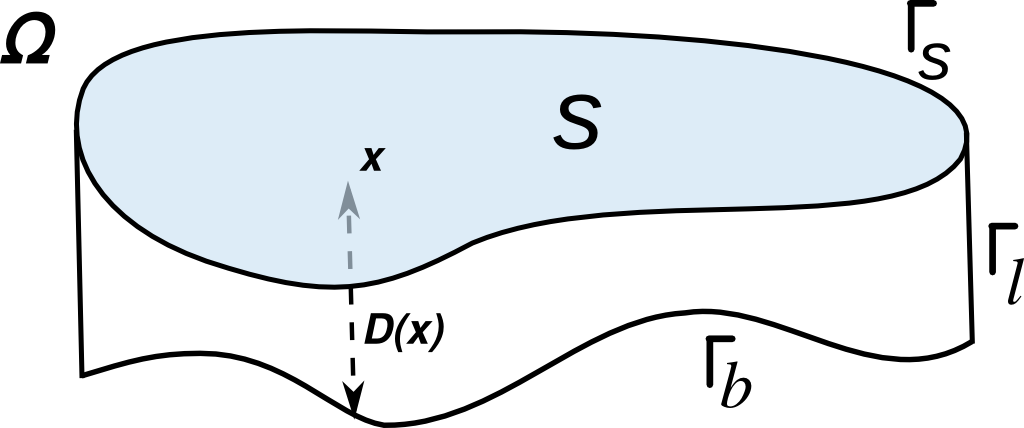
\includegraphics[width=0.4\textwidth]{img/domain}
% %    \end{center}
% %    \begin{itemize}
% %      \setlength\itemsep{1em}
% %    \item \alert{Rigid lid hypothesis} (flat surface) is introduced
% %    \item
% %      \color{darkgray} Notation:
% %      \begin{itemize}
% %      \item \color{darkgray} $\surfaceBoundary$: part of the boundary corresponding to
% %        the surface
% %      \item \color{darkgray} $\bottomBoundary$: part corresponding to the bottom
% %        boundary
% %      \item \color{darkgray} $\talusBoundary$: lateral walls (if any)
% %      \end{itemize}
% %    \end{itemize}
% %  \end{frame}

% % %----------------------------------------------------------------------
% % \begin{frame}{Anisotropic equations}
% % %----------------------------------------------------------------------
% % %  \vspace{-0.2em}
% %   \note{Comment briefly the main difficulties of Navier-Stokes equations}
% %   \begin{overprint}
% %     \onslide<1>
% %     Anisotropic momentum equations (in the isotropic) domain:
% %     \onslide<2>
% %     \alert{Vertical/Horizontal aspect ratio} \tikz[na] \coordinate(LaspectRatio);
% %     \  affects vertical velocity terms!
% %     \onslide<3>
% %     \alert{Coriolis} force
% %     \tikz[na] \coordinate(Lcoriolis);
% %     \onslide<4>
% %     \alert{\textbf{Density}}: \textbf{coupling} of energy equations.
% %     \tikz[na] \coordinate(Lcoupling);
% %     \onslide<5>
% %     \textbf{We focus on \dotfill \alert{Constant density case}}
% %     \onslide<6>
% %     \textbf{We focus on \dotfill \alert{Linear steady case}}
% %   \end{overprint}
% %   \begin{block}{\small Conservation of momentum and continuity}
% %     \vspace{-0.66\baselineskip}
% %     \begin{align*}
% %       {\onslide<1-5> \dt \uu + \uu\cdot\gradx\uu + \vv\,\dz\uu  {\onslide<-6>- \visc\Delta\uu
% %       +}} {\onslide<1-4>\frac 1 \rho_\star} \onslide<-6> \gradx \pp=
% %        \tikz[na] \node (Rcoriolis) {\framedmath<3>{\fU}};
% %       \\
% %       \tikz[na] \coordinate(RaspectRatio);
% %         \framedmath<2>{ \varepsilon^2 \Big( {\onslide<1-5> \dt \vv + \uu\cdot\gradx\vv +
% %           \vv\,\dz\vv} {\onslide<-6> - \visc\Delta\vv \Big) }}
% %         \displaystyle
% %         + {\onslide<1-4> \frac 1 \rho_\star } {\onslide<-6> \dz \pp} +
% %         {\onslide<1-4> \frac{1}{\rho_\star}} \tikz[na] \coordinate(RcouplingA);
% %           \framedmath<4>{\rho}\,\gravity {\onslide<-6> = 0\hskip+0.5em}
% %       \\[-0.2em]
% %       \div\uu + \dz\vv = 0\hskip+0.5em
% %     \end{align*}
% %     \vspace{-1.4\baselineskip}
% %   \end{block}
% %   \begin{block}<4>{\small Convection-diffusion of \textit{temperature} and
% %       \textit{salinity} + state equation (density)}
% %     \vspace{-0.66\baselineskip}
% %     \begin{align*}
% %       \dt \Te  + (\uu \cdot \gradx) \Te + (\vv\cdot\dz) \Te  - \nu_\Te\Delta \Te &= \fT
% %       \\[0.3em]
% %       \dt \Sa  + (\uu \cdot \gradx) \Sa + (\vv\cdot\dz) \Sa -
% %       \nu_\Sa\Delta \Sa &= \fS
% %       \\[0.3em]
% %       \tikz[na] \coordinate(RcouplingB);
% %       \framedmath<4>{\rho} = \rho_\star\big(1-\beta_\Te(\Te-\Te_\star) + \beta_\Sa(\Sa&-\Sa_\star)\big)
% %     \end{align*}
% %     \vspace{-1.4\baselineskip}
% %   % \item Equation of state (dependence of density in terms of
% %   %   temperature and salinity)
% %   %   where $\Te_\star$ and $\Sa_\star$ are given reference values.
% %   \end{block}
% %   \tikzstyle{RaspectRatio} = [draw, circle, minimum size=.5cm, node
% %   distance=1.75cm]
% %   \tikzstyle{redcircle} = [draw, circle, color=PHDredA, node distance=3cm,
% %   minimum height=2em]

% %   \begin{tikzpicture}[overlay]
% %     \path<2>[myarrow]
% %     (LaspectRatio) edge [out=320, in=130] (RaspectRatio);
% %     \path<3>[myarrow]
% %     (Lcoriolis) edge [out=0, in=130] (Rcoriolis);
% %     \path<4>[myarrow]
% %     (Lcoupling) edge [out=0, in=135] (RcouplingA);
% %     \path<4>[myarrow]
% %     (Lcoupling) edge [out=0, in=135] (RcouplingB);
% %         % \draw<3>[->, PHDblue, ultra thick, opacity=.8] (Lboussinesq) -- (Rboussinesq);
% %         % \draw<4>[->, PHDblue, ultra thick, opacity=.8] (LbetaPlane) -- (RbetaPlane);
% %         % \draw<5>[->, PHDblue, ultra thick, opacity=.8] (LverticalScaling) -- (RverticalScaling);
% %   \end{tikzpicture}
% % \end{frame}

% %--------------------------------------------------------------------------
% \begin{frame}[allowframebreaks]{Steady Anisotropic Stokes equations}
% %--------------------------------------------------------------------------
%   \color{darkgray}{\small Now we are interested in numerical resolution of:}
%   \smallskip
%   \begin{block}{}
%     \begin{center}\large
%       \textit{\alert{flow equations with \textbf{anisotropic} vertical/horizontal viscosity coefficients}}
%     \end{center}
%   \end{block}
%   \begin{itemize}\itemsep1em
%   \item Type of equations: mixed \textbf{anisotropic} velocity/pressure problems
%   \item  E.g. in large scale Ocean dynamics, where\medskip\small
%     \begin{equation*}
%       \varepsilon = \frac{\text{vertical
%           scales}}{\text{horizontal scales}}~
%     \begin{tabular}[t]{l} is \large\textbf{small} \\[-0.2ex]
%       \tiny\it ~ $10^{-3}$, $10^{-4}$\end{tabular}
%     \quad \text{...we can even suppose } \framedmath{\varepsilon\to 0}
%   \end{equation*}
%   % \begin{flushright}
%   %   {... we can suppose $\framedmath{\varepsilon\to 0}$}
%   % \end{flushright}
%   \end{itemize}
%   % \bigskip
%    \begin{center}
%      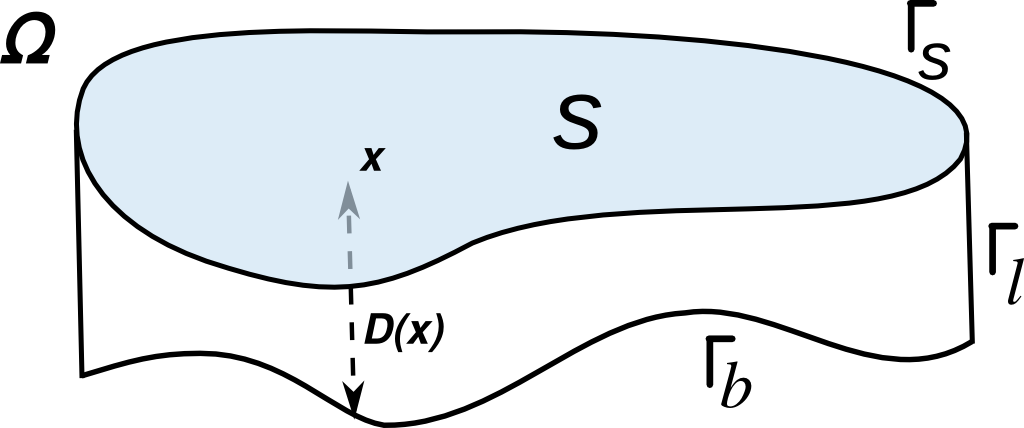
\includegraphics[width=0.4\textwidth]{img/domain}
%    \end{center}
%   \begin{block}{Steady Anisotropic Stokes equations}
%     \begin{equation*}
%       \begin{aligned}
%         - \Delta\uu + \gradx\pp &= \ff,
%         \\
%         -\framedmath{\varepsilon} \Delta\vv + \dz\pp &= g,
%         \\
%         \divx\uu + \dz\vv &= 0.
%       \end{aligned}
%     \end{equation*}
%   \end{block}

%   \begin{itemize}\itemsep1em
%   \item When $\varepsilon\to 0$, we only expect
%   $$v\in H^1_z(\Omega)=\big\{\overline v\in L^2(\Omega),
%   \dz\overline\vv\in L^2(\Omega)\big\}$$

% \item
%   Let us consider
%   the boundary conditions:
%   \begin{align*}
%     \nu\dz\uu|_{\surfaceBoundary} &= \gs,
%     \quad
%     \uu|_{\bottomBoundary\cup\talusBoundary}=0 ,
%                               % \label{eq:bc.1}
%     \\
%     \vv|_{\surfaceBoundary} &=0, \quad
%     % \intertext{adherence on bottom and talus:}
%     \vv|_{\bottomBoundary} =0,
%                              % \label{eq:bc.2}
%     \quad
%     % \intertext{and slip condition on talus:}
%     \varepsilon\gradx\vv \cdot \mathbf{n_x}|_\talusBoundary =0,
%                                                               % \label{eq:bc.3}
%   \end{align*}

% \item We look for $\ww=(\uu,\vv)\in\WW=\UU\times\VV$, \quad $\pp\in\PP$,
%   \begin{align*}
%     \UU&=\Uspace=\Big\{\uu\in \big[H^1(\Omega)\big]^{d-1} {: \ }
%          \uu|_{\bottomBoundary\cup\talusBoundary}=0\Big\},
%          % \label{eq:Uspace}
%     \\
%     \VV&=\Vspace =\Big\{\vv\in L^2(\Omega){: \ } \dz\vv\in L^2(\Omega),\
%         \vv|_{\surfaceBoundary\cup\bottomBoundary}=0\Big\},
%         % \label{eq:Vspace}
%     \\
%     \PP&=\Pspace=\Big\{\pp\in L^2(\Omega){: \ } \int_\Omega\pp=0
%          \Big\}.
%          % \label{eq:Pspace}
%   \end{align*}
% \end{itemize}
% \end{frame}


% %--------------------------------------------------------------------------
% \begin{frame}{Variational Formulation}
% %--------------------------------------------------------------------------
%   \small
% Find
% $(\uu,\vv,\pp)\in\UU\times\VV\times\PP$ such that
% \begin{equation*}
%   \begin{aligned}
%     (\grad\uu,\grad\buu) - (\pp, \divx\buu) &= (\ff,\buu) + (\gs,\buu)_{\Gamma_s}    &\ \forall\,\buu\in\UU,
%     % \label{eq:non-HS.weak.a}
%     \\
%     \varepsilon (\grad\vv,\grad\bv) - (\pp,\dz\bv) & = 0 &  \ \forall\,\bv\in\VV,
%     % \label{eq:non-HS.weak.b}
%     \\
%     (\div(\uu,\vv),\bp) &= 0 &\ \forall\,\bp\in\PP.
%     % \label{eq:non-HS.weak.c}
%   \end{aligned}
% \end{equation*}
% \note[item]{We emphasize that formulation is purely differential and,
%   unlike most usual formulations for Primitive Equations, it avoids
%   vertical integration and also avoids hypotheses of the type
%   $D(\xx)>D_0>0$. Consequently, it facilitates the use of standard (not necessarily structured) meshes and also tools and techniques
%   like mesh adaptivity.}
% \begin{theorem}
%   Anisotropic Stokes equations are well-posed (uniformly when $\varepsilon\to 0$)
% \end{theorem}
% Well posedness hinges on the following inf-sup conditions:
% \begin{alignat}{4}
%   \tag*{\ensuremath{(IS)^\PP}}
%   &\ &
%   \ConstISp \|\pp\|_0 &\le
%   \sup_{0\neq(\uu,\vv)\in \UU \times \VV}
%   \frac{(\div(\uu,\vv),\pp)}{\|(\grad \uu,\, \dz \vv)\|_0}
%   &\qquad &
%   \forall \,\pp \in \PP,
%   \label{eq:ISp}
%   \\\noalign{\smallskip}
%   \tag*{\ensuremath{(IS)^\VV}}
%   &\ &
%   \ConstISv \|\dz\vv\|_0 &\le
%   \sup_{0\neq \pp \in \PP}
%   \frac{(\dz \vv,\pp)}{\|\pp\|_0}
%   &\qquad &
%   \forall\, \vv\in \VV,
%   \label{eq:ISv}
% \end{alignat}
% \pause \alert{Discrete approximations} must verify \alert{discrete
%   versions} of \ref{eq:ISp}, \ref{eq:ISv}
% \end{frame}

% %--------------------------------------------------------------------------
% \begin{frame}{Not Easy Task!}
% %--------------------------------------------------------------------------
%   \begin{center}
%       \begin{tabular}[b]{r}
%         Classical $\P2/\P1$ FE,
%         Velocity
%         \\[1ex]
%         \alert{$\framedmath{\varepsilon=10^{-2}}$}
%         \\
%         \rule{0pt}{0.5\textheight}
%       \end{tabular}
%       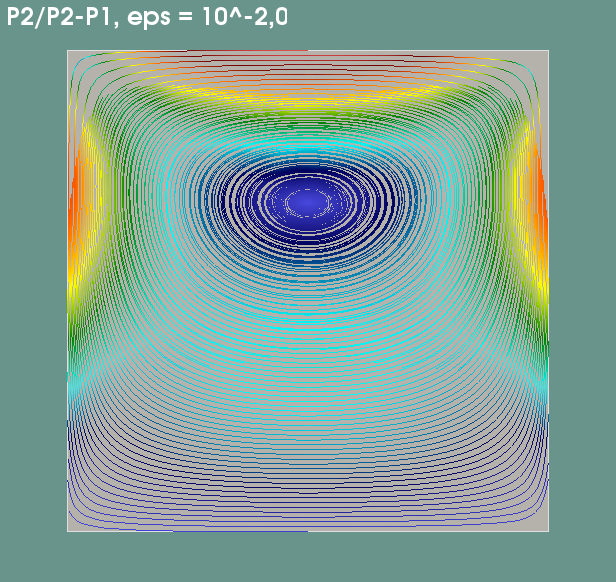
\includegraphics[width=0.5\linewidth]{img/221-eps-2}
%   \end{center}
% \vfill
% \end{frame}

% %--------------------------------------------------------------------------
% \begin{frame}{Not Easy Task!}
% %--------------------------------------------------------------------------
%   \begin{center}
%       \begin{tabular}[b]{r}
%         Classical $\P2/\P1$ FE,
%         Velocity
%         \\[1ex]
%         \alert{$\framedmath{\varepsilon=10^{-3}}$}
%         \\
%         \rule{0pt}{0.5\textheight}
%       \end{tabular}
%       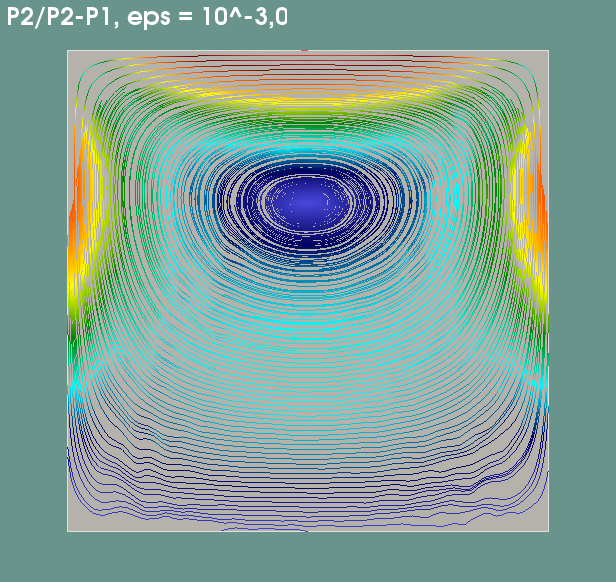
\includegraphics[width=0.5\linewidth]{img/221-eps-3}
%   \end{center}
% \vfill
% \end{frame}

% %--------------------------------------------------------------------------
% \begin{frame}{Not Easy Task!}
% %--------------------------------------------------------------------------
%   \begin{center}
%       \begin{tabular}[b]{r}
%         Classical $\P2/\P1$ FE,
%         Velocity
%         \\[1ex]
%         \alert{$\framedmath{\varepsilon=10^{-4}}$}
%         \\
%         \rule{0pt}{0.5\textheight}
%       \end{tabular}
%       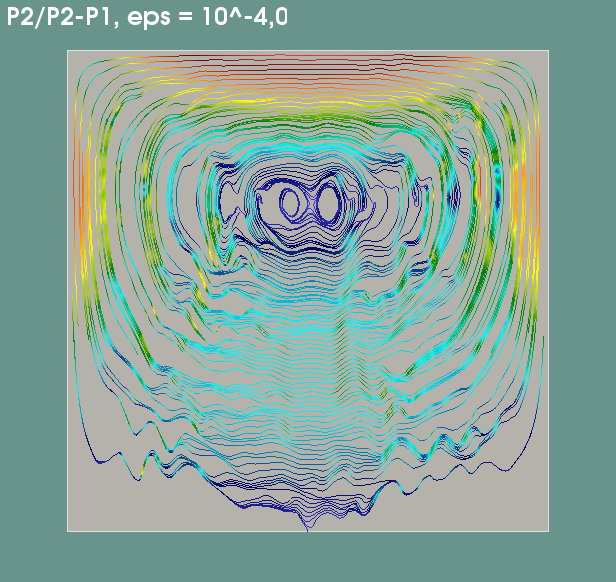
\includegraphics[width=0.5\linewidth]{img/221-eps-4}
%   \end{center}
% \vfill\pause
% \begin{center}
%   \alert{
%     \textbf{Idea}: to use DG \quad \Pd k -- \Pd k \quad approximations for Velocity--Pressure!
%   }
% \end{center}
% \end{frame}


% % ============================================================================
% \section[Introduction]{SIP-DG Approximation of Anisotropic Stokes Equations}
% % ============================================================================

% \begin{frame}{Definitions}
%   \alert{Discrete Spaces}:
% \begin{align*}
%   \UUh &= \big[\Pd{k}\big]^{d-1}, \quad \Vh=\Pd{k}, \quad \WWh=\UUh\times\Vh=\big[\Pd{k}\big]^d
%   \\[1ex]
%   \Pho &= \Pd{k}\cap L_0^2(\Omega)
% \end{align*}

% \alert{Bilinear form}:
% \vspace{-0.5em}
% \begin{equation*}
%   % \label{eq:bilinear.a}
%   a_h^{\rm anis}(\wwh,\bwwh) =  \sum_{i=1}^{d-1} \asip[sip , \eta](u_i,\overline u_i)
%   +\varepsilon \, \asip[sip , \eta](\vh,\bvh)
%   + (1-\varepsilon) \shv(\vh,\bvh)
% \end{equation*}
% where
% \begin{equation*}
%   \shv(\vh,\bvh) =
%   \sum_{e\in\Eh} \frac1{h_e} \int_e \Big(
%     \jump{\vh\nz}\jump{\bvh\nz} \Big).
% \end{equation*}
% % \vspace{-1.5em}
% \small
% \begin{itemize}
% \item Generalization of $a^{\rm Sto}(\cdot,\cdot)$  \quad $(\varepsilon=1)$
% \end{itemize}
% \end{frame}

% \begin{frame}{Properties}
%   \begin{itemize}

% \item \alert{Boundedness of $a_h^{\rm anis}(\cdot,\cdot)$}
%   \medskip
%   \begin{align*}
%     % \label{eq:asip.vh.boundedness}
%     a_h^{\rm anis}(\wwh,\bwwh)  \le C_{\rm bnd}\big( \normsip{\uuh}\normsip{\buuh} +
%     \varepsilon\, \normsip{\vh}\normsip{\bvh} \big)
%     \\ \notag
%     +  (1-\varepsilon) |\vv_h|_V |\bv_h|_V .
%   \end{align*}

%   \item
%   \alert{$\varepsilon$--dependent Coercivity of $a_h^{\rm anis}(\cdot,\cdot)$}
%   \medskip
%   For all $\eta>\eta_*$,
%   \begin{equation*}
%     % \label{eq:uv.partial.coercivity}
%     a_h^{\rm anis}(\wwh,\wwh) \ge
%     C(\eta) \big(\normsip{\uuh}^2
%     + \varepsilon  \normsip{\vh}^2  \big)
%     + (1-\varepsilon)|\vh|_V^2
%   \end{equation*}
%   where %$C(\eta)$ is given in Lemma \ref{le:asip.coercivity} and
%   \begin{equation*}
%     % \label{eq:vh_V.bound}
%     |\vh|_V^2 = \sum_{e\in\Eh} \frac1{h_e} \int_e
%     \jump{\vh \nz}^2 .
%   \end{equation*}
%   % where $C_{\eta}^{\varepsilon}=(\eta- \varepsilon \eta_*)/(1+\eta).$
%   % \label{lemma:eps.dependent.coercivity}

%   \pause
%   \alert{But we need some way for bounding $\vh$ uniformly on $\varepsilon$}!
% \end{itemize}

% \end{frame}

% \begin{frame}{Inf-sup for bounding $\dzh\vh$}
%    \bigskip
% \begin{lemma}
%    For every $\vh\in\Vh$, it holds
%   \begin{equation*}
%     % \label{eq:vh.stability}
%       \norm[0]{\dzh\vh - \mean{\dzh\vh} } =
%     \sup_{\bph \in \Pho}\frac{\int_{\Omega} \bph \, \partial_{z,h}\,\vh}{\|\bph\|_{0}},
%   \end{equation*}
%     where $\mean{\dzh\vh}$ is the mean of $\dzh\vh$ in $\Omega$.
%   % \label{lemma:vh.stability}
% \end{lemma}
% % \begin{proof}
% %   Given $\vh\in\Vh$,
% %   \nuevo{
% %     and using that $\int_{\Omega} \bph \, \mean{\dzh\vh}=0$ for any $\bph \in \Pho $,
% %   \begin{equation*}
% %     \sup_{\bph \in \Pho}\frac{\int_{\Omega} \bph \, \partial_{z,h}\,\vh}{\|\bph\|_{0}} =
% %     \sup_{\bph \in \Pho}\frac{\int_{\Omega} \bph \left(\partial_{z,h}\,\vh - \mean{\dzh\vh}\right)}{\|\bph\|_{0}}.
% %   \end{equation*}
% %  Therefore, it suffices to note that the supreme on the right hand side
% %   is reached for $\bph= \partial_{z,h} \vh - \mean{\dzh\vh}\in \Pho$.
% %   }
% % \end{proof}

% \bigskip
% % $\Rightarrow$
% \alert{\textbf{Good}!} \par
% \begin{center}
% Our \alert{discrete spaces} verify some kind of discrete~\alert{\ref{eq:ISv}}
% \\[0.33em]
% \small (hydrostatic  inf-sup condition)
% \\[1em]
% \normalsize
% At this point, \textbf{stability} (uniformly
% on~$\varepsilon\to 0$) hinges on a \\
% \alert{bound of $\norm[0]{\ph}$}. % The
% \end{center}
% \end{frame}

% \begin{frame}{Inf-sup for $\ph$}
% \begin{lemma} There exists $\ConstISph > 0$ independent of $h$, such that
%   \begin{equation*}
%     \ConstISph  \,
%       \norm[0]{\ph}
%     \le \sup_{\wwh \in \WWh \setminus \{0\}} \frac{b_h^{\rm Sto} ( \wwh, \ph )}{\structure{\normveleps{\wwh}}}
%     + | \ph |_P , \quad \forall \ph \in \Pho.
%     \label{eq:ph.stability}
%   \end{equation*}
%   \label{lemma:ph.stability}
% \end{lemma}
% Where
% \begin{equation}  \label{w-anis-norm}
%  \structure{\normveleps{\wwh}} = \left(\normsip{\uuh}^2 + \alert{\normveleps{\vh}^2}\right)^{1/2},
% \end{equation}
% being
% \small
%  $$
%  \alert{\normveleps{\vh}^2}
%  =\varepsilon \|\nabla_{{\bf x},h} v_h\|_0^2 + \alert{\norm[0]{\dzh\vh}}^2
% + \sum_{e\in\Eh} \frac1{h_e} \int_e \Big( \varepsilon\jump{\vh \nx}^2+\alert{\jump{\vh \nz}}^2  \Big).
% $$


% \end{frame}


% \begin{frame}{Anisotropic DG Scheme}
%   Discretization of the Anisotropic Stokes
%   problem:\medskip
%   \par\hfill {\small find $(\wwh, \ph) \in \WWh \times \Pho$ such that}
% \alert{
% \begin{equation*}
%   \begin{aligned}  % \label{disc-var-pb.a}
%   a_h^{\rm anis} ( \wwh, \bwwh) +b_h^{\rm Sto} ( \bwwh, \ph )
%   &= \int_{\Omega}\! \ff \cdot \buuh
%    \!+\! \int_{\Gamma_s}\! \gs \cdot \buuh,
%   \\  % \label{disc-var-pb.b}
%   -b_h^{\rm Sto} (\wwh, \bph) + s_h^p (\ph, \bph)
%   % + \pEpsilon
%   %   \int_\Omega \ph\bph
%   &=0,
% \end{aligned}
% \end{equation*}
% }
% \hfill {\small\color{gray} $\forall \,\bwwh=(\buuh,\vh) \in \WWh$  \ and \  $\forall\, \bph \in \Pho$}.

% Or equivalently
% \alert{
% \begin{equation*}
%   c_h^{\rm anis} \big ( (\wwh,\ph), ( \bwwh, \bph) \big )=\displaystyle\int _{\Omega} \ff \cdot \buuh
%   + \int_{\Gamma_s} \gs\cdot\buuh , \
%   % \label{eq:hydrostatic.reformulation}
% \end{equation*}
% }
% \hfill {\color{gray}\small $\forall (\bwwh, \bph) \in \WWh \times \Pho$}

% {\small
%   Where
% \begin{multline*}
% c_h^{\rm anis} \big( (\wwh,\ph), ( \bwwh, \bph) \big)= a_h^{\rm anis} ( \wwh, \bwwh)
% +b_h^{\rm Sto} ( \bwwh, \ph )
% \\
% -b_h^{\rm Sto} (\wwh, \bph) + s_h^p (\ph, \bph). % +\pEpsilon\int_\Omega \ph \bph.
% \label{eq:bilinear.c}
% \end{multline*}
% }
% \end{frame}

% \begin{frame}{Well-Posedness of SIP-DG Anisotropic Stokes}
% We consider  the following norm in $\Xh =\WWh \times \Pho$:
% \begin{equation*}
%   \| (\wwh, \ph)\|^2_{\varepsilon,\Xh} = \normveleps{{\bf w}_h}^2 + \| \ph
%   \|_{0}^2 + |\ph|_P^2
% %   =
% %   \\
% %   \normsip{\uuh}^2
% %   +
% % \normveleps{\vh}^2
% %   + \| \ph \|_{0}^2 + |\ph|_P^2.
%   % =
%   % \normsip{\uuh}^2
%   % \\
%   % +\varepsilon\norm[0]{\gradxh\vh}^2 + \norm[0]{\dzh\vh}^2 +
%   %   \seminormVeps{\vh}^2
%   %  + \| \ph \|_{0}^2 + |\ph|_P^2.
% \end{equation*}
% \begin{theorem}[Inf-Sup Stability]
%   \label{teor.well-posedness}
%   Assume that that $ \eta > \eta_*$. Then,
%   there exists $\gamma >0$ independent of $h$ such that, for all
%   $(\wwh, \ph) \in \Xh= \WWh \times \Pho$, one has
%   \begin{equation}
%     \label{eq:global.inf-sup}
%       \gamma \,\| (\wwh, \ph)\|_{\varepsilon,\Xh}
%     \le \sup_{(\bwwh,\bph)\in \Xh \setminus
%       \{0\}} \frac{c_h^{\rm anis} ( (\wwh, \ph), (\bwwh,\bph)  ) }{\norm[\varepsilon,\Xh]{(\bwwh,\bph)} }.
%   \end{equation}
% \end{theorem}
% According to Banach-Necas-Babu\v{s}ka Theorem we have:
% %
% \begin{corollary}
% Well-Posedness of SIP-DG-Stokes
% \end{corollary}

% \end{frame}
% % %--------------------------------------------------------------------------
% % \begin{frame}{Instability of \textit{Classical} Finite Elements}
% % %--------------------------------------------------------------------------
% %   \begin{itemize}
% %     \itemsep=1.2em
% %   \item ``Classical'' Taylor-Hood $\P2/\P1$ F.E. \textbf{not stable} when $\varepsilon\to 0$
% %   \item Similar results for bubble $\P{1,b}/\P1$ F.E.
% %   \item Why? \ \ One has stokes-like inf-sup condition...
% %     \par\hfill\uncover<2->{\alert<2>{and also a \textbf{new hydrostatic inf-sup condition}}}
% %     \begin{alignat*}{4}
% %       \label{eq:ISp}
% %       \tag*{\ensuremath{(IS)^\PP}\xspace}
% %       &\quad&
% %       \sup_{0\neq(\uu,\vv)\in \UU \times \VV}
% %       \frac{(\div(\uu,\vv),\pp)}{\|\grad \uu,\dz \vv\|}
% %       &\ge \ConstISp \|\pp\|
% %       &\quad&
% %       \forall \pp \in \PP,
% %       \\[1.0em]
% %       \label{eq:ISv}
% %       \onslide<2->
% %       \tag*{\ensuremath{(IS)^\VV}\xspace}
% %       &\quad &
% %       \alert<2>{
% %         \sup_{0\neq \pp \in \PP}
% %         \frac{(\dz \vv,\pp)}{\|\pp\|}}
% %       &\alert<2>{\ge \ConstISv \|\dz\vv\|}
% %       &\quad&
% %       \alert<2>{\forall \vv\in \VV}
% %     \end{alignat*}
% %   \item<3> New inf-sup condition means:
% %     \begin{center}
% %       \structure{\# dofs($\alert{v}$)} not bigger than \structure{\#
% %         dofs($\alert{p}$)}
% %     \end{center}
% %   \end{itemize}
% % \end{frame}




% % %---------------------------------------------------------------------
% % \begin{frame}{Partial $\varepsilon$--dependent Coercivity}
% % % ---------------------------------------------------------------------
% %   \begin{itemize}
% %     \itemsep=1em
% %   \item For \underline{$\uuh$}, coercivity of SIP bilinear form yields:
% %     \begin{equation*}
% %       \sum_{i=1}^{d-1} \asip[sip , \eta](u_i,\overline u_i) \ge
% %       C(\eta) \normsip{\uuh}^2 \quad
% %       \structure{\scriptsize=\quad C(\eta) \sum_{i=1}^{d-1}\normsip{u_i}^2}
% %     \end{equation*}
% %   \item
% %     For \underline{$(\uuh,\vh)$} we can show:
% %     \begin{lemma}[$\varepsilon$--dependent coercivity]
% %       For all $\eta>\eta_*$ and for all $\wwh=(\uuh,\vh) \in \WWh$,
% %       \begin{equation*}
% %         a_h(\wwh,\wwh) \ge C(\eta) \Big(
% %         \normsip{\uuh}^2
% %         + \varepsilon  \norm[0]{\gradh\vh}^2
% %         % + C_{\eta}^{\varepsilon}\seminormVeps{\vh}^2
% %         + \seminormVeps{\vh}^2
% %         \Big),
% %       \end{equation*}
% %       where
% %       $$
% %       \seminormVeps{\vh}^2 = \sum_{e\in\Eh} \frac1{h_e} \int_e\Big(
% %       \varepsilon\jump{\vh\nx}^2 + \jump{\vh \nz}^2 \Big).
% %       $$
% % \end{lemma}
% % \end{itemize}
% % \begin{scriptsize}
% % \hfill \textit{Proof}:
% %   (1) write $\asip[\varepsilon](\vh,\bvh)$ in terms of
% %     $\varepsilon\asip[sip , \eta](\vh,\bvh)$,\enspace (2) apply coercivity of $\asip[sip , \eta](\vh,\bvh)$
% % \end{scriptsize}
% % \end{frame}

% % %---------------------------------------------------------------------
% % \begin{frame}{Partial $\varepsilon$--dependent Coercivity II}
% % % ---------------------------------------------------------------------
% %   \begin{itemize}
% %     \itemsep=0.75em
% %   \item The norm used in previous Lemma degenerates when $\varepsilon\to 0$
% %   \item We redefine it, introducing $\framedmath{\dzh\vh}$:
% %     \begin{align*}
% %       \alert{\normsip{\vh}{_{,\varepsilon}}}= \left( \varepsilon\norm[0]{\gradxh\vh}^2 + \framedmath{\norm[0]{\dzh\vh}^2} +
% %       \seminormVeps{\vh}^2\right)^{1/2},
% %       \\[0.5em]
% %       \text{and consider}\enspace \normveleps{\wwh} = \left(\normsip{\uuh}^2 + \alert{\normsip{\vh}}^2{_{,\varepsilon}}\right)^{1/2}.
% %     \end{align*}
% %   \item And we have an \textit{hydrostatic} inf-sup condition for $\framedmath{\dzh\vh}$:
% % \begin{lemma} [Inf-Sup stability for $\dzh\vh$]
% %   \begin{equation}
% %     \tag*{\ensuremath{(IS)^\Vh}\xspace}
% %     \norm[0]{\dzh\vh} =
% %     \sup_{\bph \in \Ph}\frac{\int_{\Omega} \bph \, \partial_{z,h}\,\vh}{\|\bph\|_{0}}
% %     \quad \forall\vh\in\Vh.
% %   \end{equation}
% %   \label{lemma:vh.stability}
% % \end{lemma}
% %   \end{itemize}
% % \end{frame}

% \section{Numerical Tests}
% \label{sec:numerical-tests}

% \begin{frame}{\textbf{Cavity tests} for Anisotropic Equations}
%   \textbf{Aim}: \alert{test qualitative behavior of DG solution when $\varepsilon \to 0$}
%   \begin{itemize}
%   \item FreeFem++
%   \item $\Omega=(0,1)^2$, mesh: $h\simeq 1/30$
%   \item Dirichlet boundary conditions:
%     \begin{itemize}
%     \item \alert{Surface} boundary:
%       $\Gamma_s$: $\uh=x(1-x)$ and $\vh=0$
%     \item \alert{Bottom}: ($\Gamma_b$): $\uh=0$ and $\vh=0$
%     \item Lateral \alert{walls}: ($\Gamma_l$): $\uh=0$
%     \end{itemize}
%   \item Neumann boundary conditions on lateral \alert{walls} $\Gamma_l$:
%     $\varepsilon\grad\vh\cdot\nn=0$
%   \item SIP DG, $\Pd{1}$, interior penalty: $\eta=5$.
%   \item As usual in DG methods, Dirichlet boundary conditions are
%     \textbf{\alert{imposed weakly}}
%     \begin{itemize}
%     \item {\color{gray} Specifically, for each jump and mean boundary
%         term appearing in DG bilinear forms, we add a corresponding
%         term to the RHS containing the boundary value}
%     \end{itemize}
%   \end{itemize}
% \end{frame}


% \newcommand{\graphHratio}{0.47}
% \newcommand{\graphVratio}{0.47}

% \begin{frame}{\textbf{Test 1}. Anisotropic equations, $\varepsilon=1$ (Stokes case)}
% \begin{center}
%   \begin{tabular}[c]{cc}
%     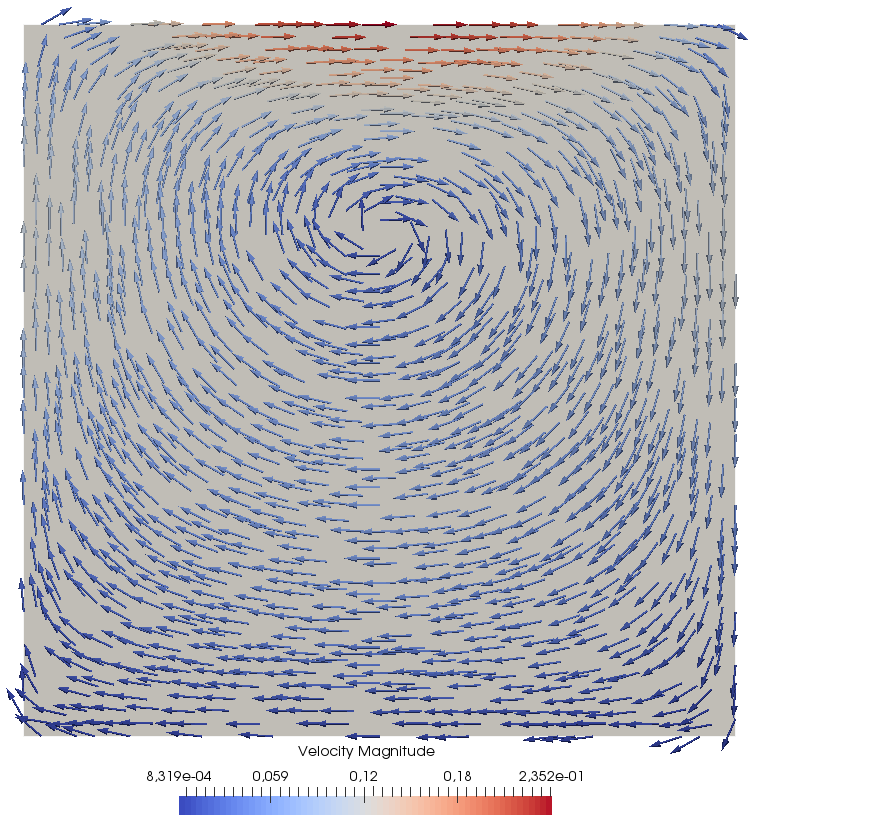
\includegraphics[
%     width=\graphHratio\linewidth,
%     height=\graphVratio\linewidth
%     ]{img/v-eps1}
%     &
%     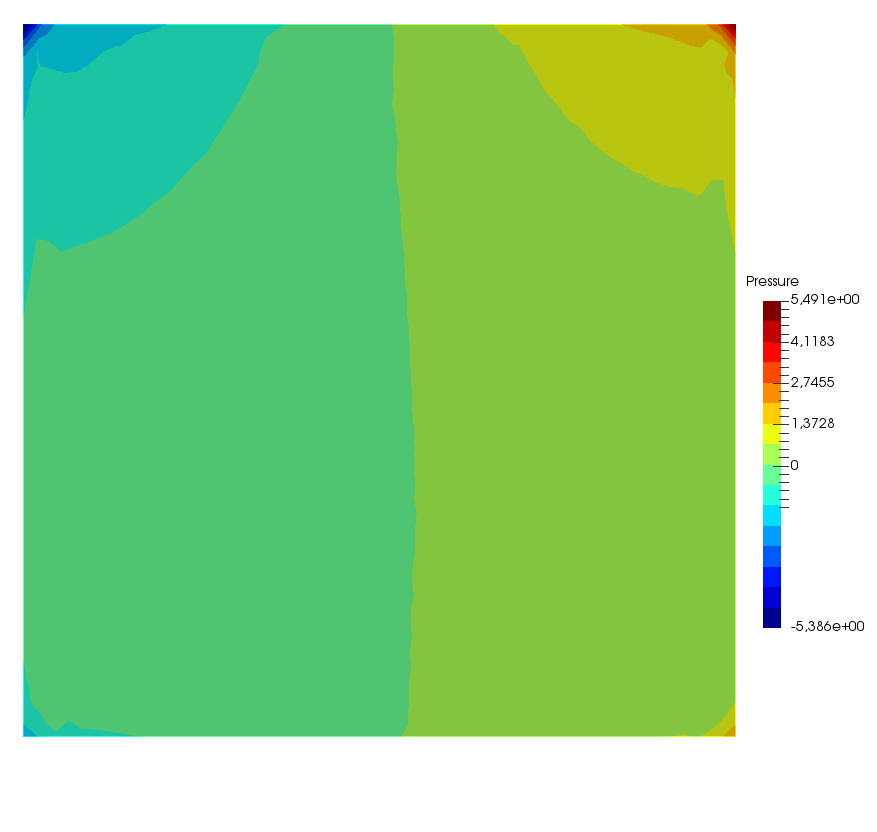
\includegraphics[
%     width=\graphHratio\linewidth,
%     height=\graphVratio\linewidth
%     ]{img/p-eps1}
%   \end{tabular}
%   \\[1em]
%   \textbf{Figure 1.} Cavity test, $\varepsilon=1$.
% \end{center}
% \end{frame}

% \begin{frame}{\textbf{Test 2}. Anisotropic equations, $\varepsilon=10^{-8}$ and $\varepsilon=0$ (Hydrostatic case)}
% \begin{center}
%   \begin{tabular}[c]{cc}
%     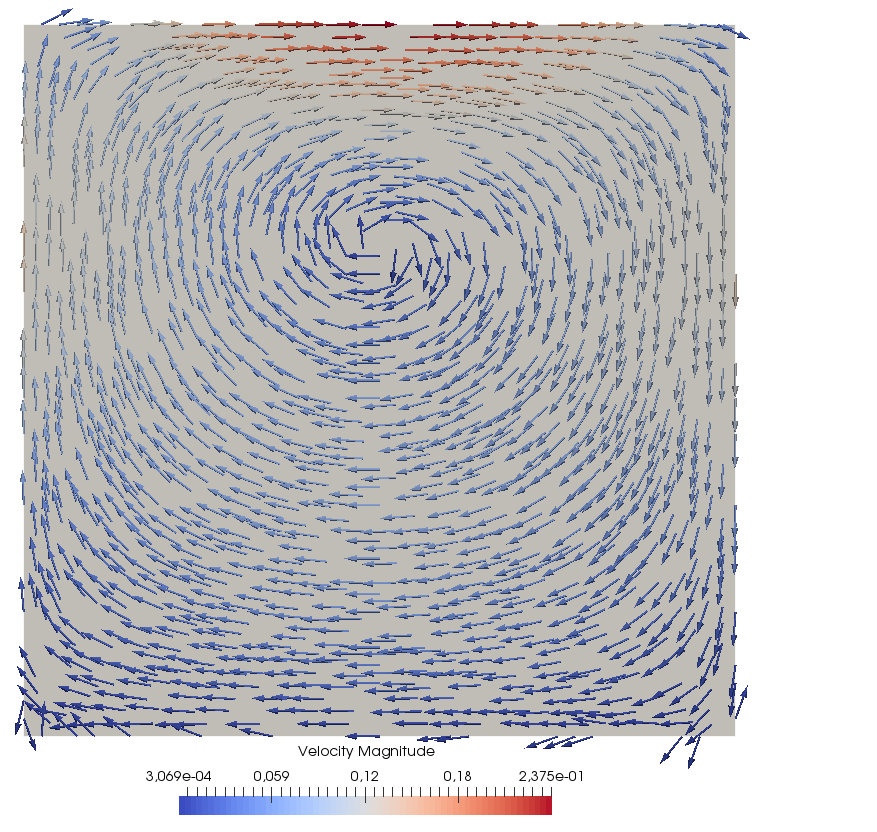
\includegraphics[
%     width=\graphHratio\linewidth,
%     height=\graphVratio\linewidth
%     ]{img/v-eps0}
%     &
%     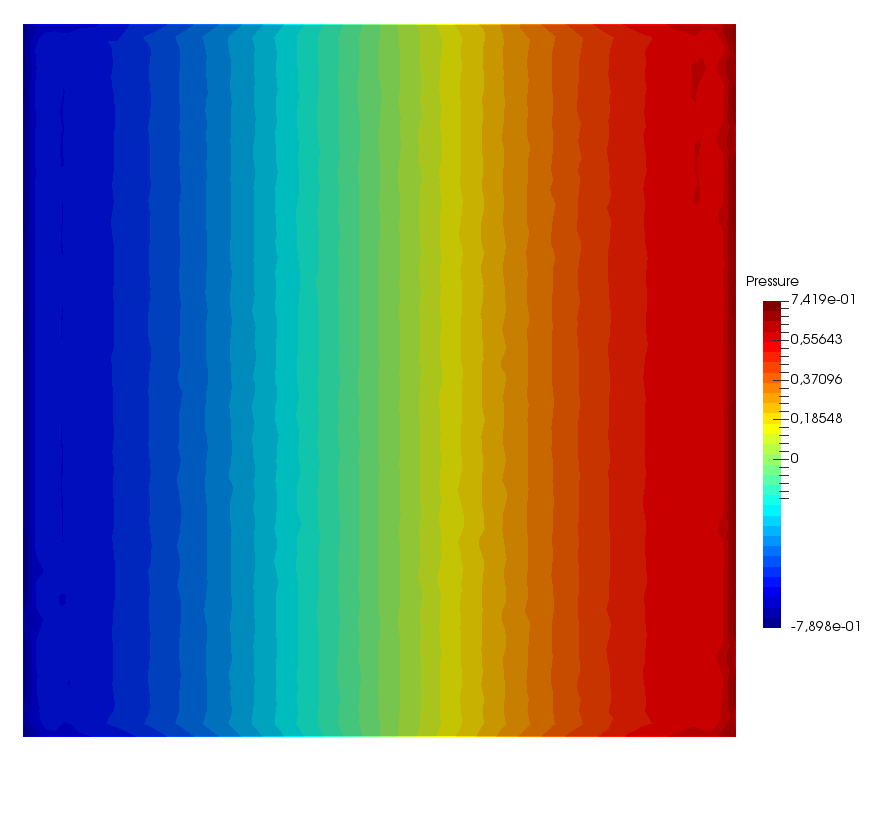
\includegraphics[
%     width=\graphHratio\linewidth,
%     height=\graphVratio\linewidth
%     ]{img/p-eps0}
%   \end{tabular}
%   \\[1em]
%   \textbf{Figure 2.} Cavity test, $\varepsilon=10^{-8}$ and $\varepsilon=0$.
% \end{center}
% \end{frame}

% \renewcommand{\graphHratio}{0.33}
% \renewcommand{\graphVratio}{0.33}
% \begin{frame}{\textbf{Test 3}. Necessity of Anisotropic Term}
% \begin{center}
%   \begin{tabular}[c]{@{}c@{}c@{}c@{}}
%     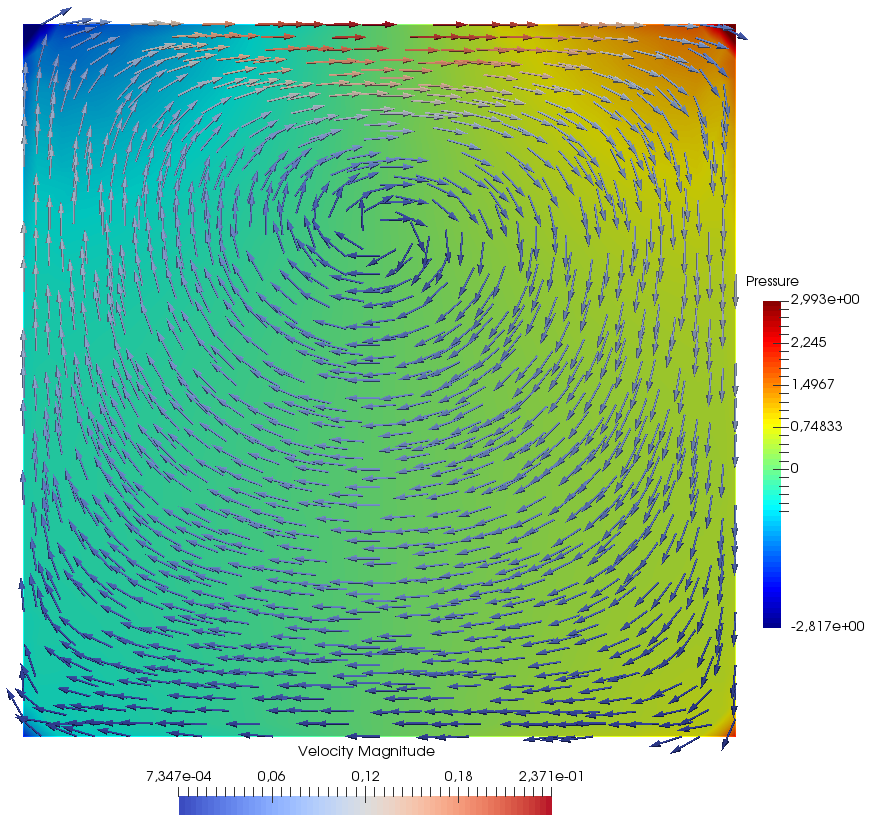
\includegraphics[
%     width=\graphHratio\linewidth,
%     height=\graphVratio\linewidth
%     ]{img/test-eps0}
%     &
%     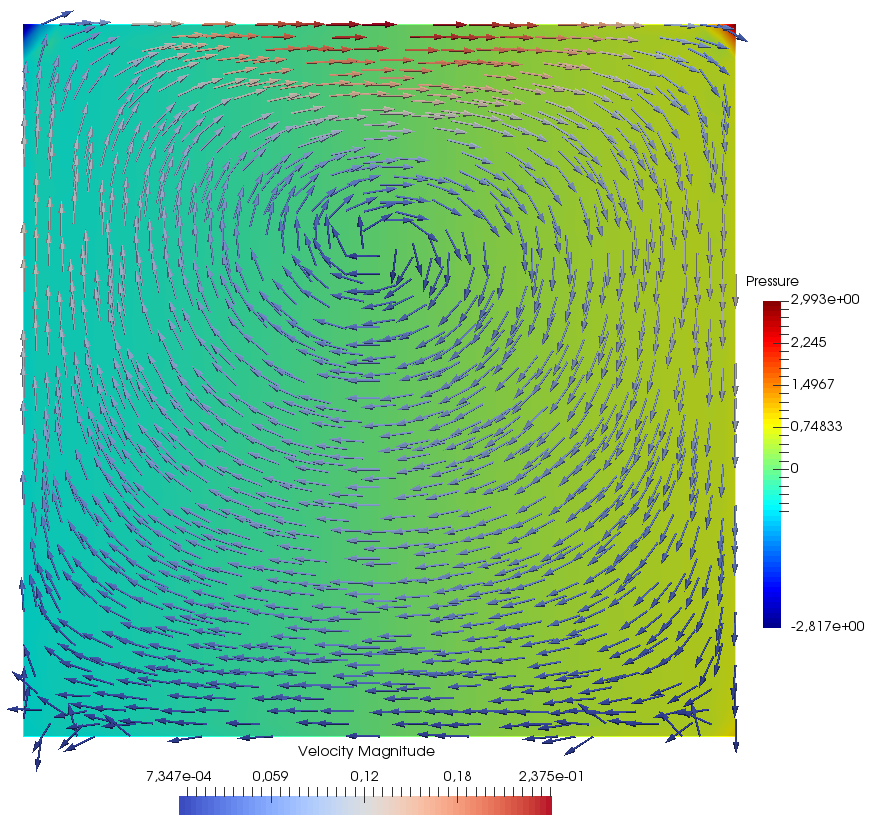
\includegraphics[
%     width=\graphHratio\linewidth,
%     height=\graphVratio\linewidth
%     ]{img/test-eps1e-1}
%     &
%     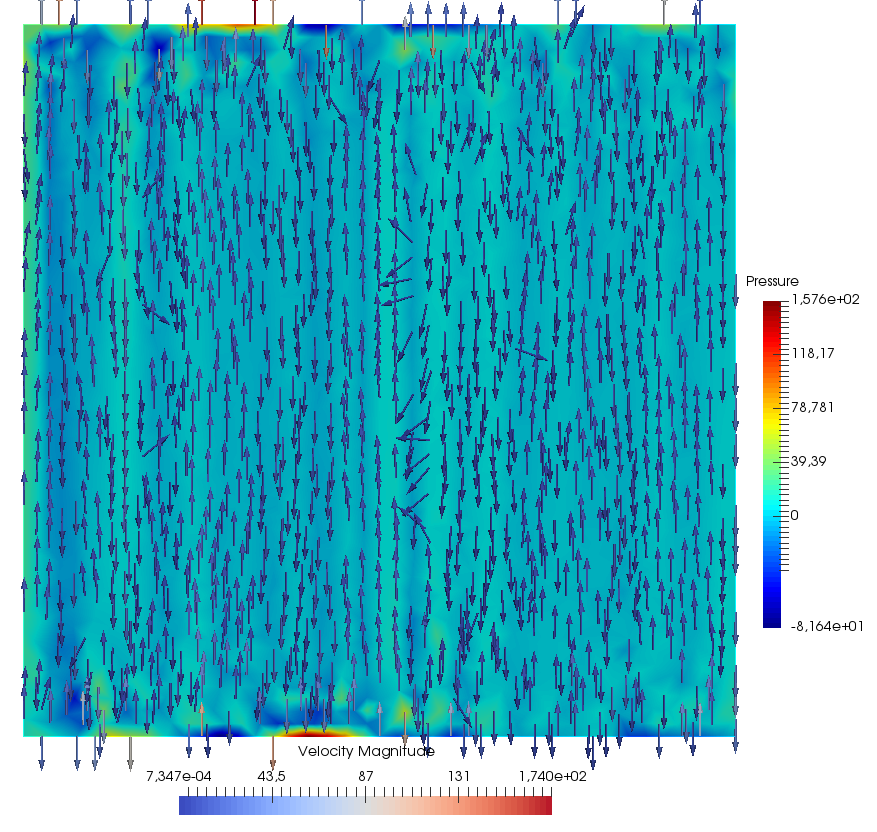
\includegraphics[
%     width=\graphHratio\linewidth,
%     height=\graphVratio\linewidth
%     ]{img/test-eps1e-2}
%   \end{tabular}
%   \\[1em]
%   \textbf{Figure 3.} Anisotropic DG scheme, \alert{without}
%   the term \alert{$(1-\varepsilon) \shv(\vh,\bvh)$} for $\varepsilon=1$,
%   $\varepsilon=10^{-2}$ and $\varepsilon=10^{-4}$, respectively.
% \end{center}
% \end{frame}

% % %---------------------------------------------------------------------
% % \begin{frame}{DG Bilinear Form for Anisotropic Stokes}
% % % ---------------------------------------------------------------------
% %   \medskip
% %   \small
% %   % \begin{itemize}
% %     % \itemsep=1em
% %   % \item
% %   \structure{\bf Order \underline{$k$} polynomials for \underline{\textit{velocity}} and \underline{\textit{pressure}}}: \llaveizq{$\wwh=(\uuh,v_h)\in\WWh$, \\
% %     $\ph \in \Ph$,}
% %     \begin{align*}
% %       \WWh&=\UUh\times\Vh=(\Pd k)^d, \quad \UUh = (\Pd k)^{d-1}, \quad \Vh=\Pd k
% %       \\
% %       \Ph &= \Pd k.
% %     \end{align*}
% %     % For each $\wwh=(\uuh,\vh)$ and $\bwwh=(\buuh,\bvh) \in\WWh$, with
% %     % $\uuh=(u_i)_{i=1}^{d-1}$ and $\buuh=(\overline u_i)_{i=1}^{d-1}$,
% %   % \item
% %     \medskip
% %     \structure{\bf Anisotropic velocity bilinear form}: \enspace
% %     $\forall \wwh=(\uuh,\vh),\ \bwwh=(\buuh,\bvh) \in\WWh$,
% %     \begin{equation*}
% %       a_h(\wwh,\bwwh) = \Big( \sum_{i=1}^{d-1} \asip[sip , \eta](u_i,\overline u_i)
% %       + \tikz[na] \node(Laepsilon){\framedmath<2>{\alert<2>{\asip[\varepsilon](\vh,\bvh)}}};
% %       \Big),
% %     \end{equation*}
% %     \vspace{-0.5em}
% %     \onslide<2>
% %     where
% %     \begin{multline*}
% %       \alert{\framedmath<2>{\asip[\varepsilon](\vh,\bvh)} =\tikz[na] \coordinate (Raepsilon);}
% %       \\
% %       \alert{ \varepsilon \,\asip[sip, 0](\vh,\bvh)
% %       + \eta\sum_{e\in\Eh} \frac1{h_e} \int_e \Big( \varepsilon
% %       \jump{\vh\nx}\jump{\bvh\nx} + \jump{\vh\nz}\jump{\bvh\nz} \Big),}
% %     \end{multline*}
% %     \begin{itemize}
% %     \item[$\star$] \scriptsize $\varepsilon$--dependent bilinear form,
% %       standard $\vh$ SIP stabilizing term is replaced by anisotropic term
% %     \item[$\star$] Generalization of previous works (for Isotropic \&
% %       Hydrostatic viscous
% %       fluids~\cite{Guillen-RedondoNeble-RGalvan:17})
% %     \end{itemize}
% %   \begin{tikzpicture}[overlay]
% %     \path<2>[myarrow] (Laepsilon) edge [out=210, in=40] (Raepsilon);
% %   \end{tikzpicture}
% % \end{frame}

% %%,---------------------------------------------------------------------
% %%|
% %%`---------------------------------------------------------------------

% %% ,---------------------------------------------------------------------
% %%| Conclusions and future work
% %%`---------------------------------------------------------------------
% \begin{frame}{Conclusions}
%   \begin{itemize}\itemsep0.66em
%   \item DG methods relax constraints of Galerkin approximate solutions to EDP's
%   \item Therefore \alert{DG methods offer new possibilities}
%   \item We have \alert{taken advantage} of them for approximation of
%     \alert{Anisotropic Stokes} equations

%   \item \textbf{\alert{Future}}: Study DG applying in other
%     topics of our interest
%     \begin{itemize}
%     \item (non-linear) Navier-Stokes equations
%     \item Solidification
%     \item Keller-Segel equations
%     \item ...
%     \end{itemize}
%   \end{itemize}
% \end{frame}

% \end{document}

% % \end{frame}
% % \begin{frame}{~}
% %   \bigskip
% %   \Large Thank you for your attention.
% %   \vfill~
% %   \begin{flushright}
% %     \pgfsetfillopacity{0.4}
% %     \pgfimage[width=0.9\textwidth]{img/gibraltar-velocity-2d-difumin}
% %   \end{flushright}
% % \end{frame}

% % %%,-------------
% % %%| Bibliography
% % %%`-------------

% % \setbeamertemplate{footline}[default]

% % \begin{frame}[allowframebreaks]{Bibliography}
% % \bibliographystyle{alpha}
% % %\bibliographystyle{abbrvnat}
% % \bibliography{biblio-short.bib}
% % \end{frame}

% \end{document}


% %%% Local Variables:
% %%% coding: utf-8
% %%% TeX-master: t
% %%% mode: latex
% %%% ispell-local-dictionary: "english"
% %%% End:
